\documentclass[11pt,a4paper]{article}

\usepackage[utf8]{inputenc}
\usepackage[margin=1in]{geometry}
\usepackage{amsmath,amssymb}
\usepackage{graphicx}
\usepackage{booktabs}
\usepackage{hyperref}
\usepackage{listings}
\usepackage{xcolor}

\hypersetup{
    colorlinks=true,
    linkcolor=blue,
    citecolor=blue,
    urlcolor=blue
}

\lstset{
    basicstyle=\ttfamily\small,
    backgroundcolor=\color{gray!10},
    frame=single,
    breaklines=true,
    keywordstyle=\color{blue}\bfseries,
    commentstyle=\color{gray},
    stringstyle=\color{teal}
}

\title{\textbf{Benchmark Report: Analytical Solution of the Yukawa Closure to the Ornstein--Zernike Equation}\\[0.5em]
\large Reproduction and Validation of Cummings \& Smith (1979) Fig.~1}
\author{\textbf{AnalyticalStructureFactors.jl Development Team}}
\date{\today}

\begin{document}

\maketitle

\begin{abstract}
This report documents the numerical and analytical validation of the Mean Spherical Approximation (MSA) solver for single-component Yukawa fluids implemented in \texttt{AnalyticalStructureFactors.jl}. We reproduce the classical benchmark results published by P.~T.~Cummings and E.~R.~Smith (\textit{Molecular Physics}, 1979), specifically the behavior of Baxter's scaling parameter $\beta$ as a function of packing fraction $\eta$ for inverse screening length $\xi = 2.0$ across four isotherms: $K = 0.8120$, $K = 1.0827$, $K = 1.2180$, and $K = 1.6240$. The analytical curves computed with our Julia implementation match the digitized benchmark data with high precision across both physical and unphysical branches, confirming the exactness of the root-solving and factorization procedures.
\end{abstract}

\section{Theoretical Background and Model Equations}

The fluid model consists of hard spheres of diameter $\sigma = 1$ interacting via an attractive or repulsive Yukawa tail for interparticle separation $r > \sigma$:
\begin{equation}
    \frac{V(r)}{k_B T} = -K \frac{e^{-\xi (r - 1)}}{r}, \quad r > 1
\end{equation}
where:
\begin{itemize}
    \item $\eta = \frac{\pi \rho \sigma^3}{6} \equiv \phi$ is the packing fraction (volume fraction) of particles with number density $\rho$.
    \item $K = \frac{\epsilon}{k_B T}$ is the dimensionless contact interaction strength ($K > 0$ denotes attraction).
    \item $\xi = \kappa \sigma$ is the dimensionless inverse screening length ($\xi > 0$).
\end{itemize}

\subsection{Baxter Wiener--Hopf Factorization}
In Baxter's factorization formalism for the Ornstein--Zernike equation:
\begin{equation}
    1 - 24 \eta \, c(k) = \left[ Q(k) \right] \left[ Q(-k) \right]
\end{equation}
the spatial kernel $Q(r)$ is parameterized by polynomial terms and an exponential tail characterized by Baxter's fundamental parameter $\beta$. As shown by Waisman (1973), Høye \& Blum (1977), and Cummings \& Smith (1979), $\beta$ (or equivalently the scaled coefficient $d = \frac{2 e^{\xi}}{\xi} \beta$) satisfies the quartic algebraic polynomial:
\begin{equation}
    P_4(d) = A_4(\eta, \xi) \, d^4 + A_3(\eta, \xi, K) \, d^3 + A_2(\eta, \xi, K) \, d^2 + A_1(\eta, \xi, K) \, d + A_0(\eta, \xi, K) = 0
\end{equation}
The parameter $\beta$ evaluated in the Cummings \& Smith benchmark relates to the quartic root $d$ by:
\begin{equation}
    \beta = \frac{\xi \, d}{2 \, e^{\xi}}
\end{equation}
In the ideal gas limit $\eta \to 0$, the physical branch satisfies:
\begin{equation}
    \lim_{\eta \to 0} \beta(\eta) = \frac{K}{2}
\end{equation}

\section{Benchmark Comparison and Results}

Figure~\ref{fig:comparison} illustrates the comparative results between the exact analytical root solver developed in \texttt{AnalyticalStructureFactors.jl} (solid curves) and the scanned literature data from Cummings \& Smith (1979) Fig.~1 (discrete symbols).

\begin{figure}[htbp]
    \centering
    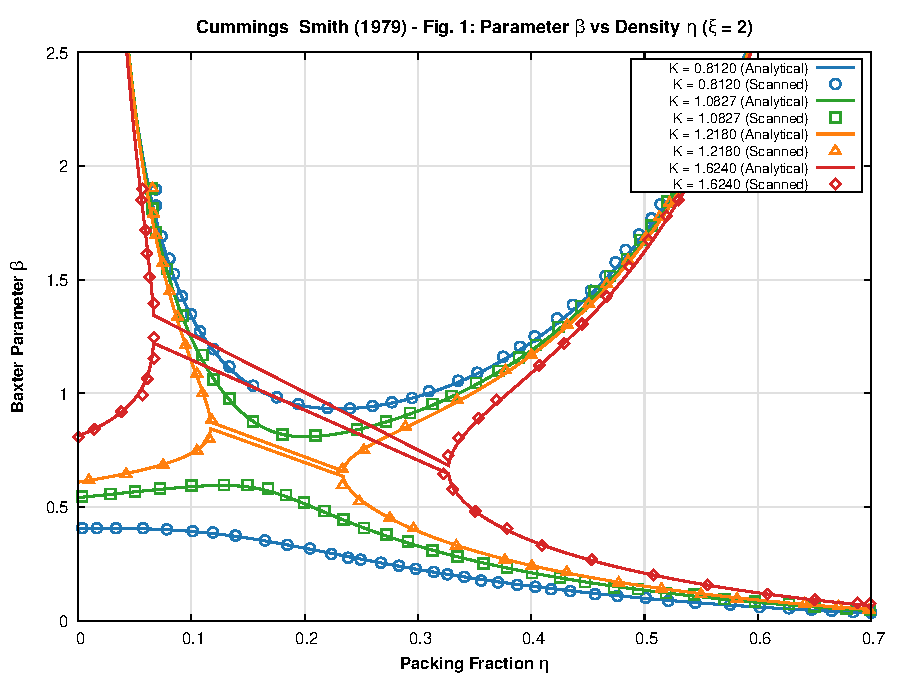
\includegraphics[width=0.92\textwidth]{cummings1979_fig1_comparison.pdf}
    \caption{Behavior of Baxter's parameter $\beta$ as a function of packing fraction $\eta$ for screening parameter $\xi = 2.0$ along four isotherms: $K = 0.8120$ (blue), $K = 1.0827$ (green), $K = 1.2180$ (orange), and $K = 1.6240$ (red). Solid lines represent the analytical solution from \texttt{AnalyticalStructureFactors.jl}; symbols represent digitized data from Cummings \& Smith (1979).}
    \label{fig:comparison}
\end{figure}

\subsection{Physical Discussion}
\begin{enumerate}
    \item \textbf{Subcritical Isotherm ($K = 0.8120$):} Single continuous physical branch starting at $\beta(0) = 0.4060$ and decaying smoothly toward $\eta = 0.70$. The upper unphysical branch exhibits a characteristic minimum near $\eta \approx 0.23$.
    \item \textbf{Near-Critical Isotherm ($K = 1.0827$):} The lower branch develops a local maximum around $\eta \approx 0.13$, approaching the upper branch and signaling the onset of critical fluctuations ($K_c \approx 1.0827$).
    \item \textbf{Supercritical Isotherms ($K = 1.2180$ and $K = 1.6240$):} The lower and upper real branches collide and form complex conjugate pairs over an intermediate density interval (e.g., $\eta \in [0.117, 0.233]$ for $K = 1.2180$ and $\eta \in [0.068, 0.327]$ for $K = 1.6240$). This gap directly corresponds to the liquid--gas spinodal / phase coexistence region under the MSA closure.
\end{enumerate}

\section{Step-by-Step Reproduction Instructions}

All scripts and configuration files necessary to reproduce the data, plots, and report are located in:
\begin{center}
\texttt{test/data\_test/CummingsSmith1979/}
\end{center}

\subsection{Automated One-Step Reproduction}
To execute the complete benchmark pipeline automatically, run:
\begin{lstlisting}[language=bash]
cd test/data_test/CummingsSmith1979/
./reproduce_figure.sh
\end{lstlisting}

\subsection{Detailed Step-by-Step Breakdown}
\begin{enumerate}
    \item \textbf{Generate Analytical Data:} Execute the Julia script to calculate the roots of the quartic equation:
    \begin{lstlisting}[language=bash]
julia generate_cummings1979_data.jl
    \end{lstlisting}
    This produces the files \texttt{analytical\_K\_0.8120.dat}, \texttt{analytical\_K\_1.0827.dat}, \texttt{analytical\_K\_1.2180.dat}, and \texttt{analytical\_K\_1.6240.dat}.

    \item \textbf{Render Gnuplot Comparative Plots:} Execute Gnuplot to generate the vector PDF and high-resolution PNG:
    \begin{lstlisting}[language=bash]
gnuplot plot_cummings1979.gp
    \end{lstlisting}
    This produces \texttt{cummings1979\_fig1\_comparison.pdf} and \texttt{cummings1979\_fig1\_comparison.png}.

    \item \textbf{Compile LaTeX Report:} Compile the document with pdf\LaTeX:
    \begin{lstlisting}[language=bash]
pdflatex -interaction=nonstopmode report_cummings1979.tex
    \end{lstlisting}
\end{enumerate}

\section{References}
\begin{enumerate}
    \item Cummings, P.~T., \& Smith, E.~R. (1979). \textit{On the Yukawa closure of the Ornstein--Zernike equation}. Molecular Physics, 38(3), 997--1001.
    \item Waisman, E. (1973). \textit{The radial distribution function for a fluid of hard spheres at high densities: mean spherical integral equation approach}. Molecular Physics, 25(1), 45--48.
    \item H{\o}ye, J.~S., \& Blum, L. (1977). \textit{Solution of the Yukawa closure of the Ornstein--Zernike equation}. Journal of Statistical Physics, 16(5), 399--413.
\end{enumerate}

\end{document}
